\documentclass[tikz,border=3pt]{standalone}
\usepackage[utf8]{inputenc}
\usepackage[T1]{fontenc}
\usepackage{lmodern}
\renewcommand{\familydefault}{\sfdefault}
\usepackage{sansmath}\sansmath
\usepackage{chemfig}
\usepackage{pgfplots}\pgfplotsset{compat=1.18,/pgf/number format/use comma,/pgf/number format/1000 sep={.}}
\usetikzlibrary{arrows.meta,calc,positioning,decorations.pathmorphing,patterns}
% paleta del sitio
\definecolor{nar}{HTML}{E8680C}\definecolor{narc}{HTML}{FFB35C}\definecolor{hielo}{HTML}{FFF3E8}
\definecolor{tinta}{HTML}{1D1D1F}\definecolor{gris}{HTML}{6E6E73}\definecolor{lila}{HTML}{7C5CF0}
\definecolor{azul}{HTML}{2F6FD6}\definecolor{menta}{HTML}{17A673}\definecolor{coral}{HTML}{E8342A}
\begin{document}
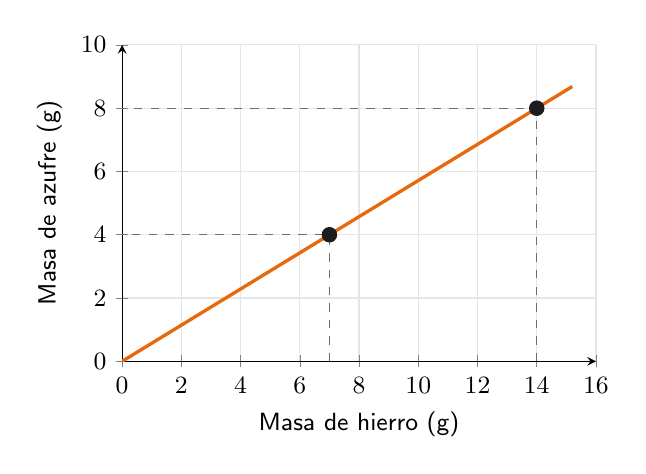
\begin{tikzpicture}
\begin{axis}[width=7.6cm,height=5.6cm,axis lines=left,xmin=0,xmax=16,ymin=0,ymax=10,xtick={0,2,...,16},ytick={0,2,...,10},
  xlabel={Masa de hierro (g)},ylabel={Masa de azufre (g)},grid=major,grid style={gray!20},tick label style={font=\small},label style={font=\small}]
\addplot[nar,very thick,domain=0:15.2] {4/7*x};
\draw[dashed,gris] (axis cs:7,0) -- (axis cs:7,4) -- (axis cs:0,4);
\draw[dashed,gris] (axis cs:14,0) -- (axis cs:14,8) -- (axis cs:0,8);
\addplot[only marks,mark=*,mark size=2.6pt,tinta] coordinates {(7,4)(14,8)};
\end{axis}
\end{tikzpicture}
\end{document}
